\chapter{Изменение точек для дивергентного поля скоростей(lagrangian)}
\label{app:div_lg}

\begin{figure}[h]
	\centering
	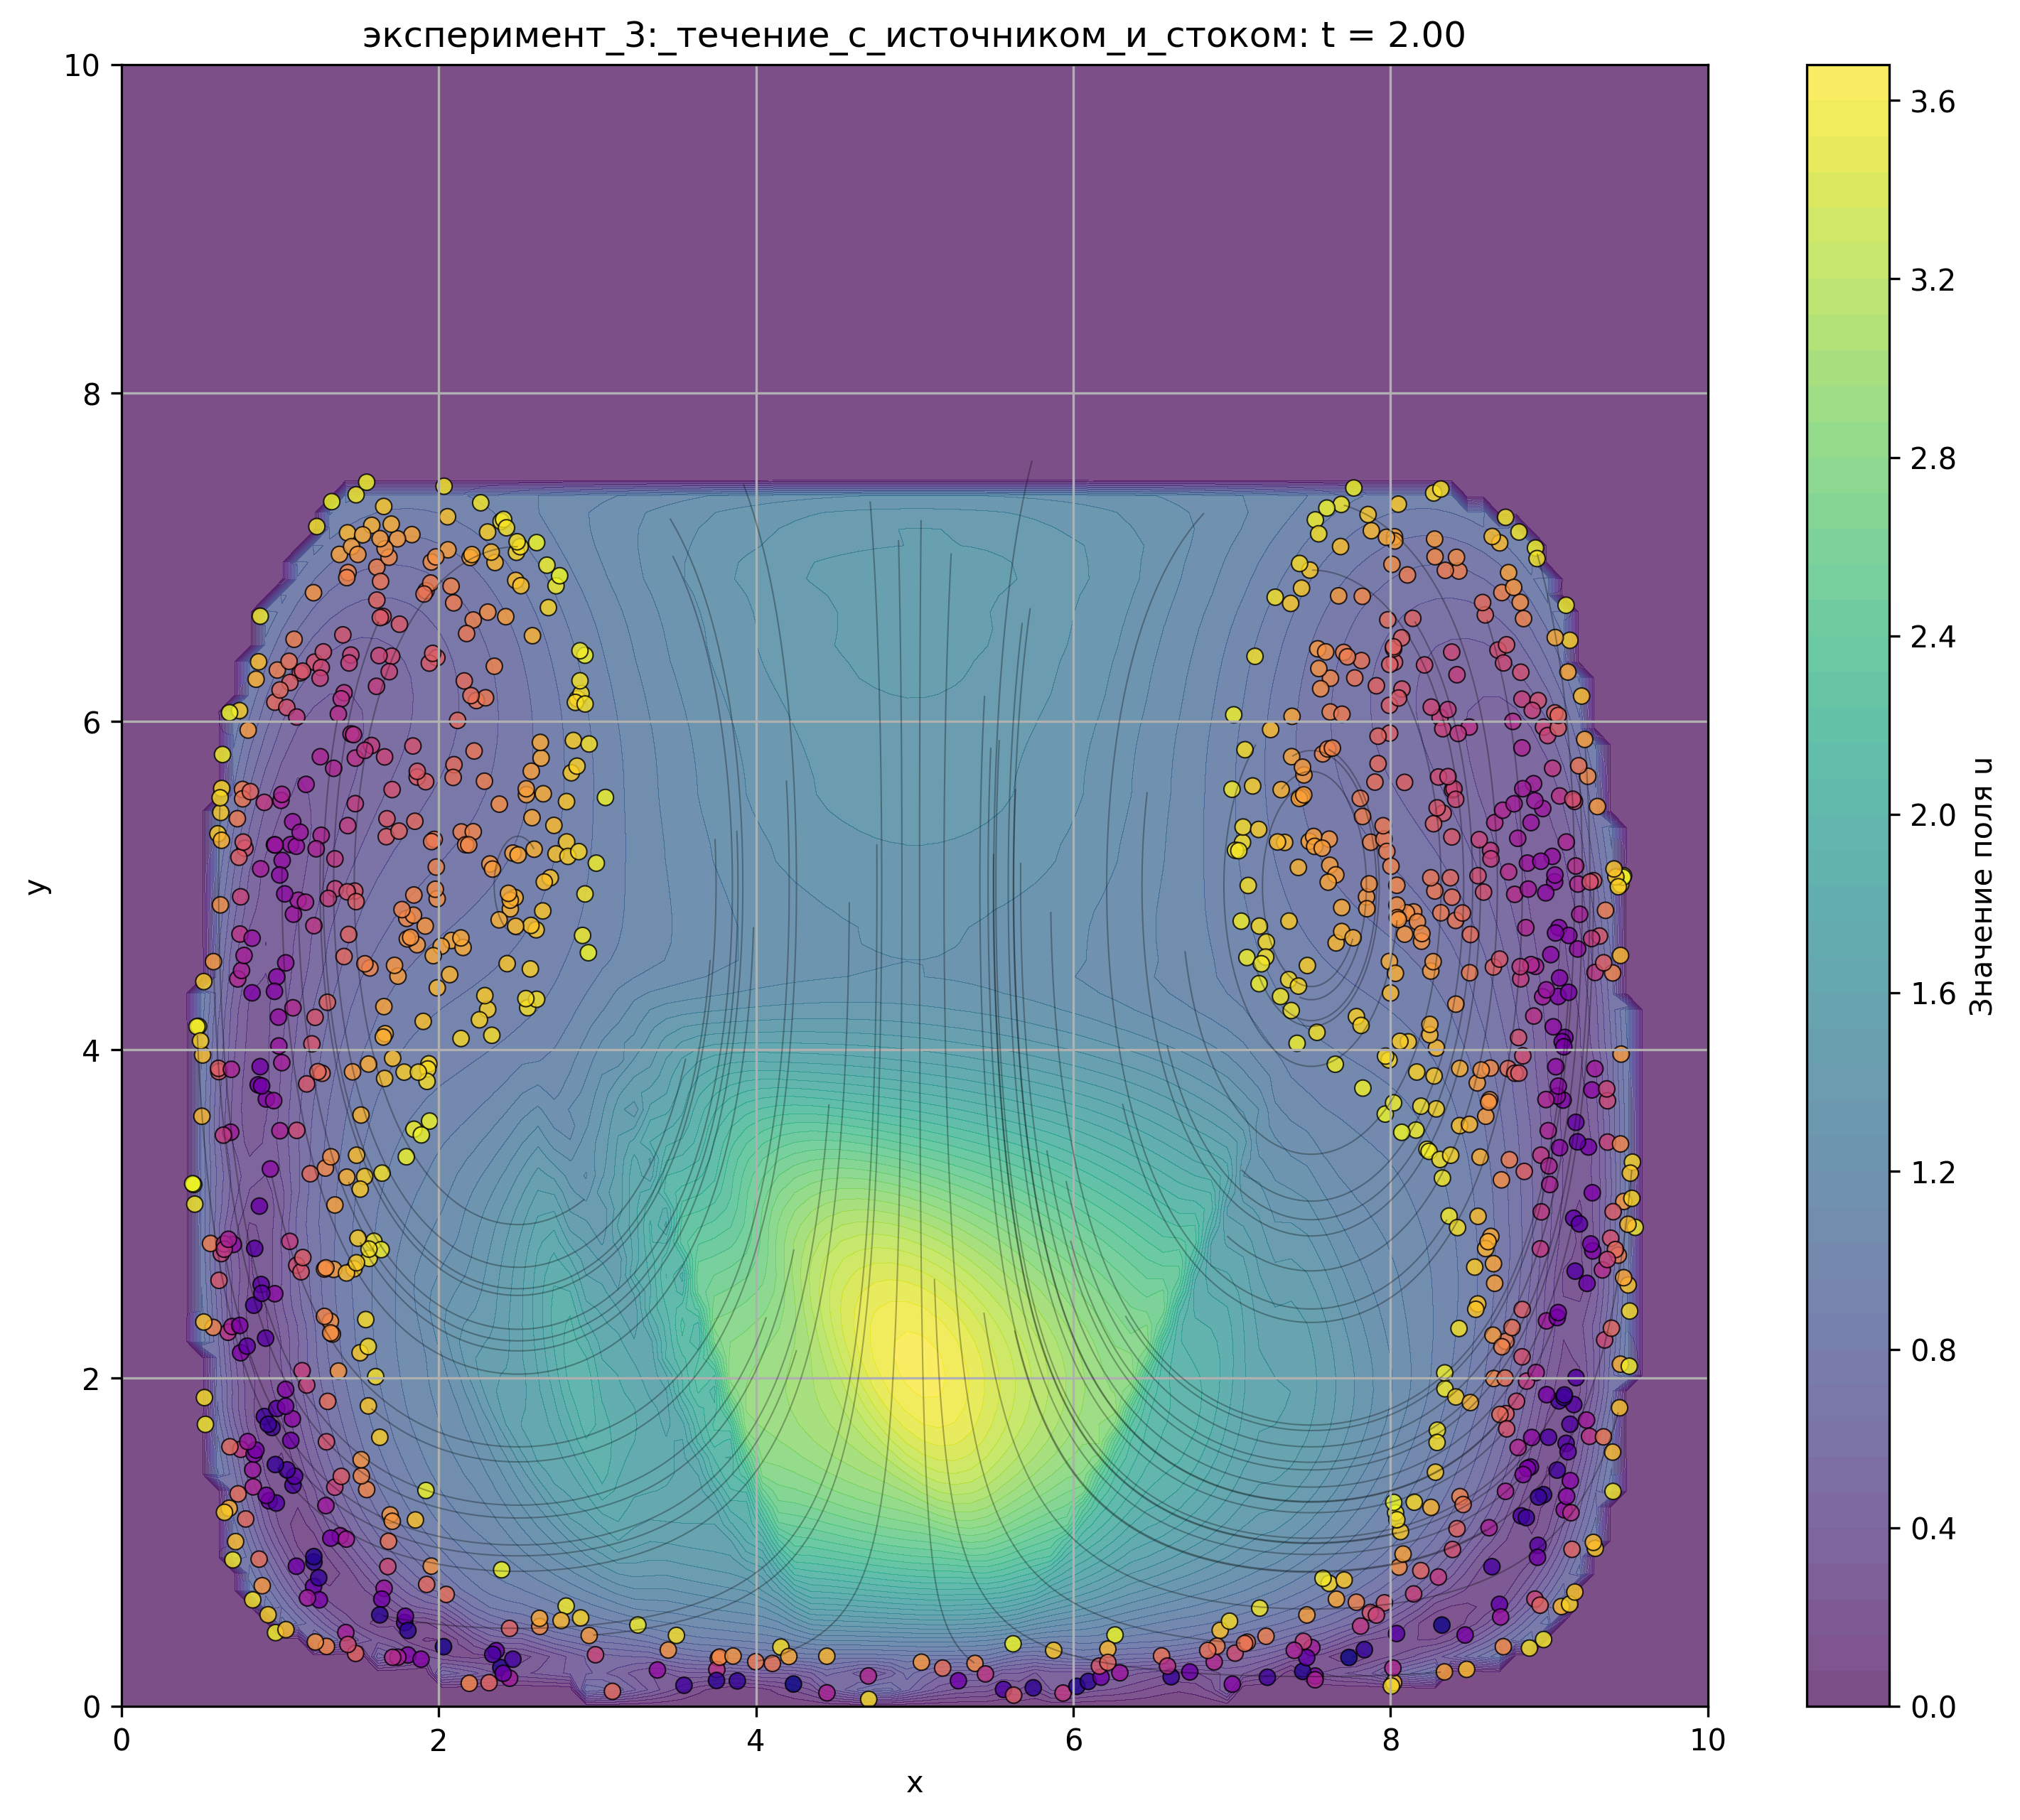
\includegraphics[width=0.6\textwidth]{imgs/lg/эксперимент_3:_течение_с_источником_и_стоком_t2.00.png}
	\caption{Скалярное поле в момент времени $t=2$ }
\end{figure}
\begin{figure}[h]
	\centering
	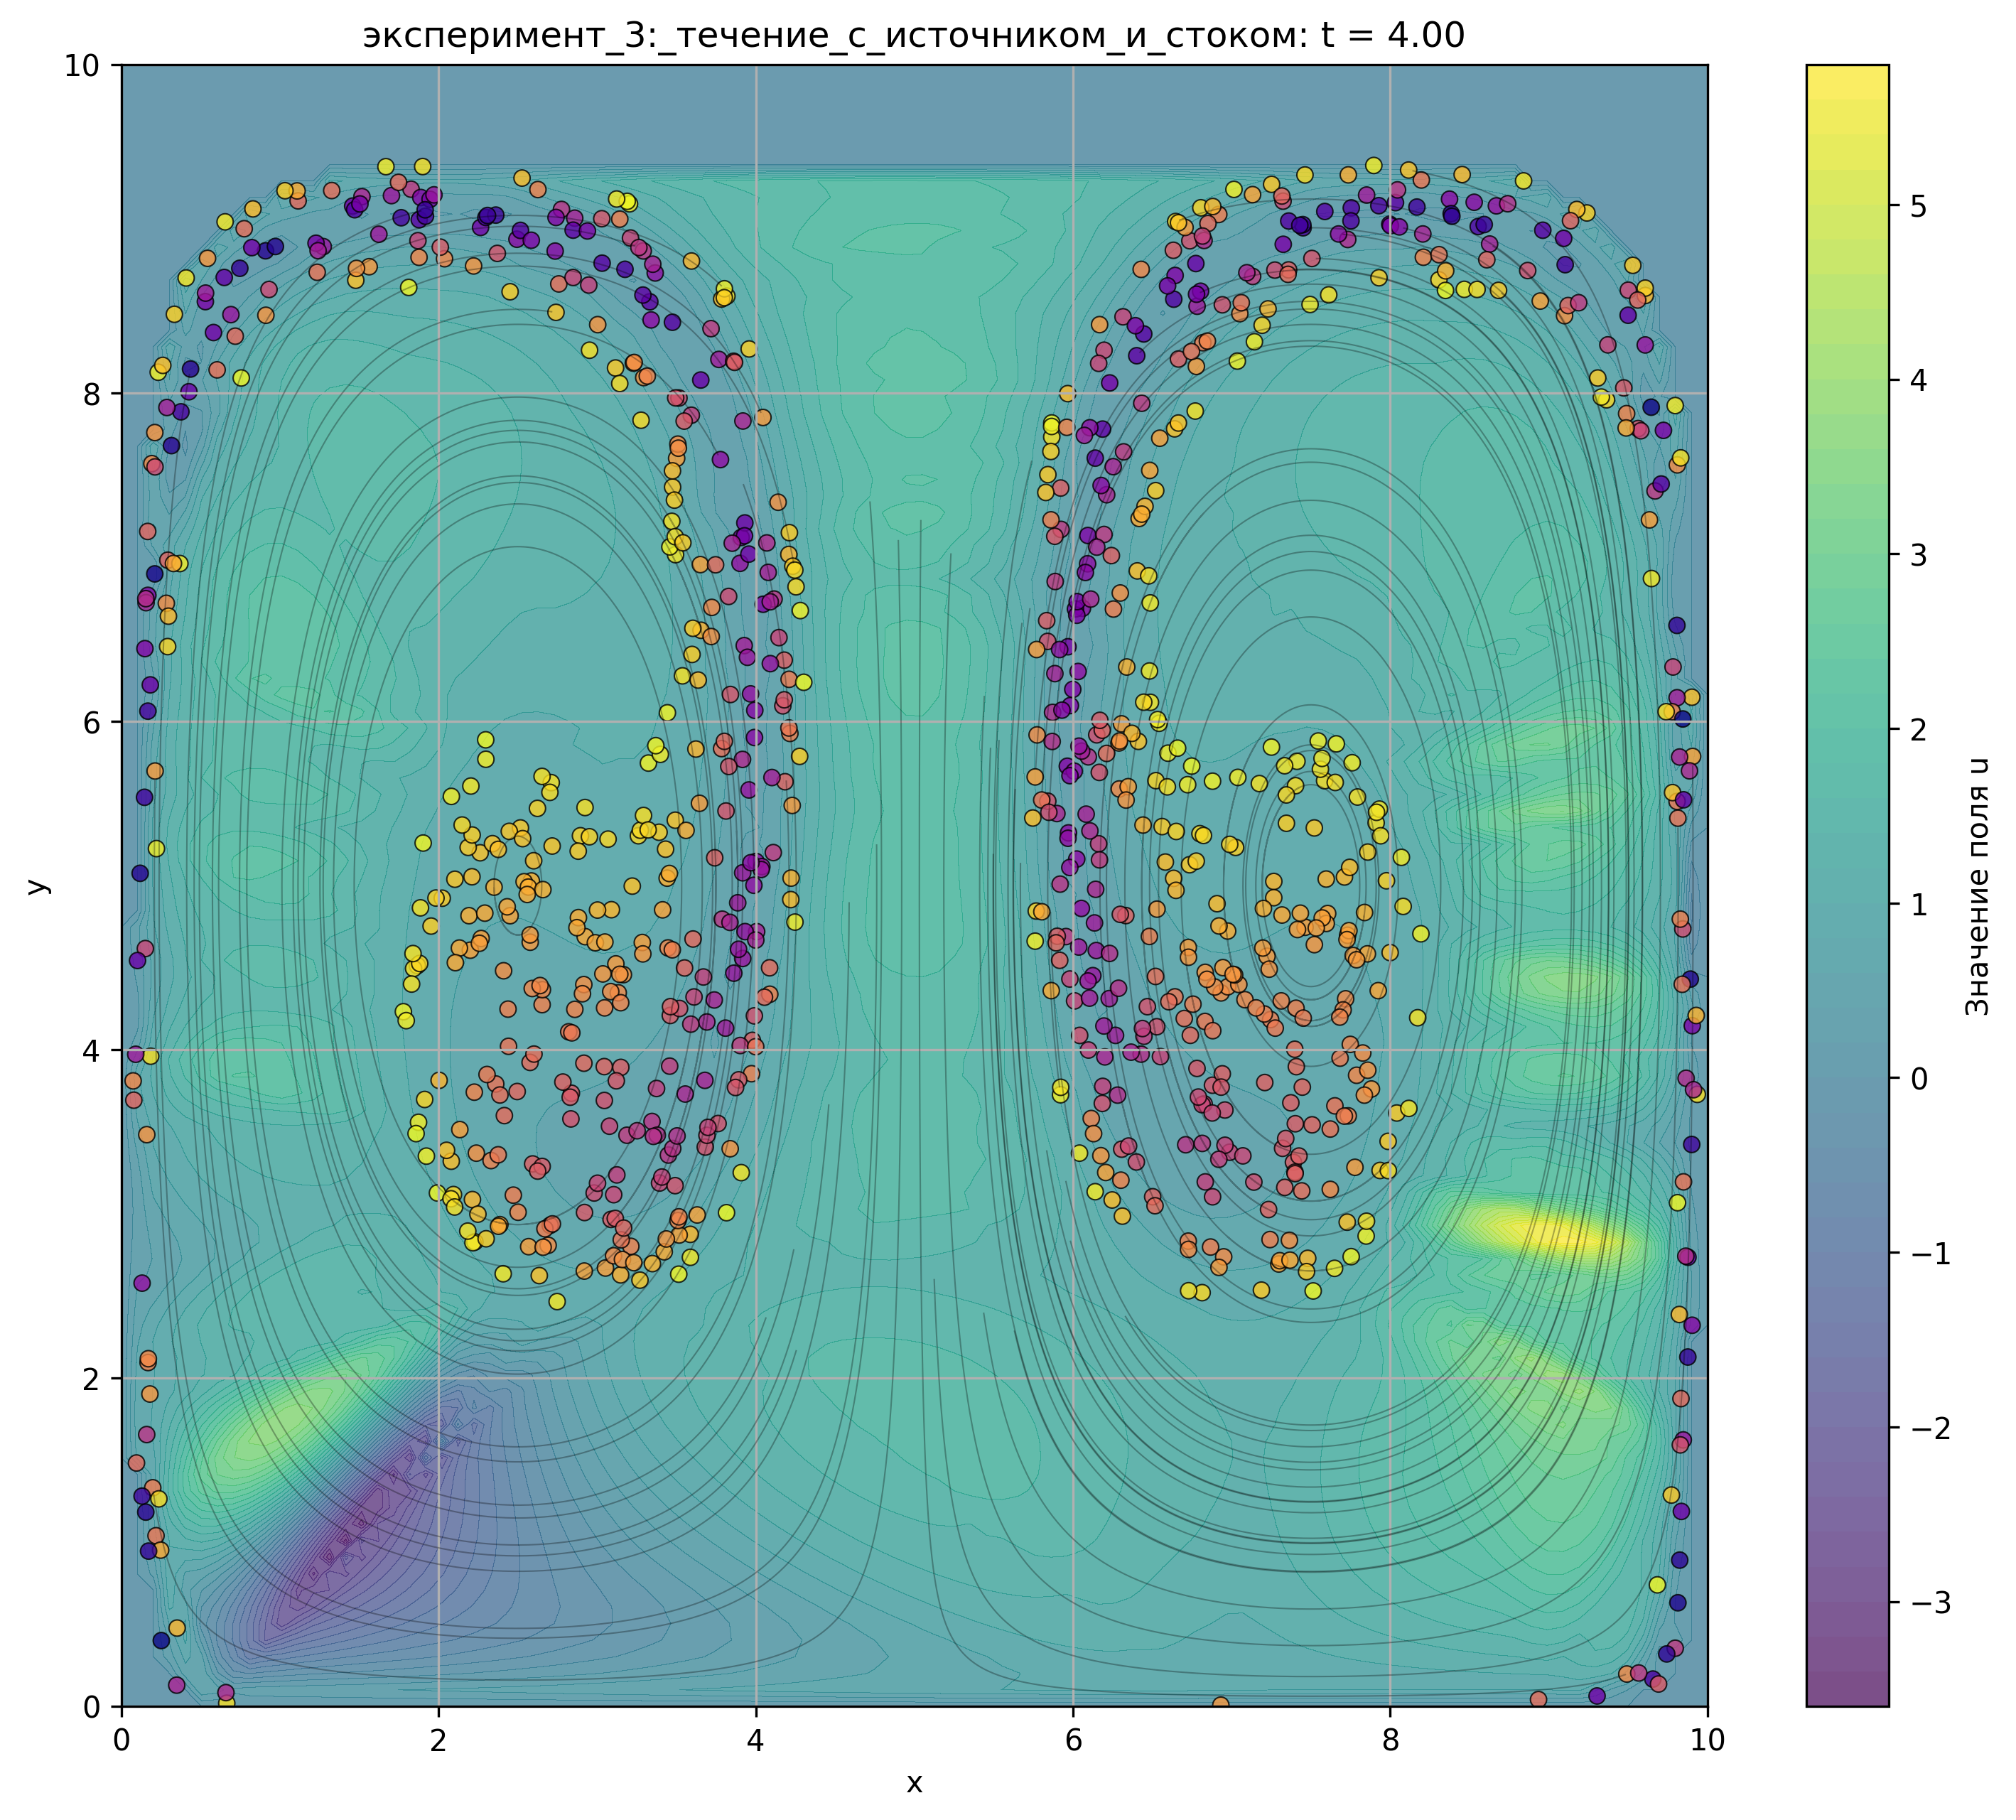
\includegraphics[width=0.6\textwidth]{imgs/lg/эксперимент_3:_течение_с_источником_и_стоком_t4.00.png}
	\caption{Скалярное поле в момент времени $t=4$}
\end{figure}
\begin{figure}[h]
	\centering
	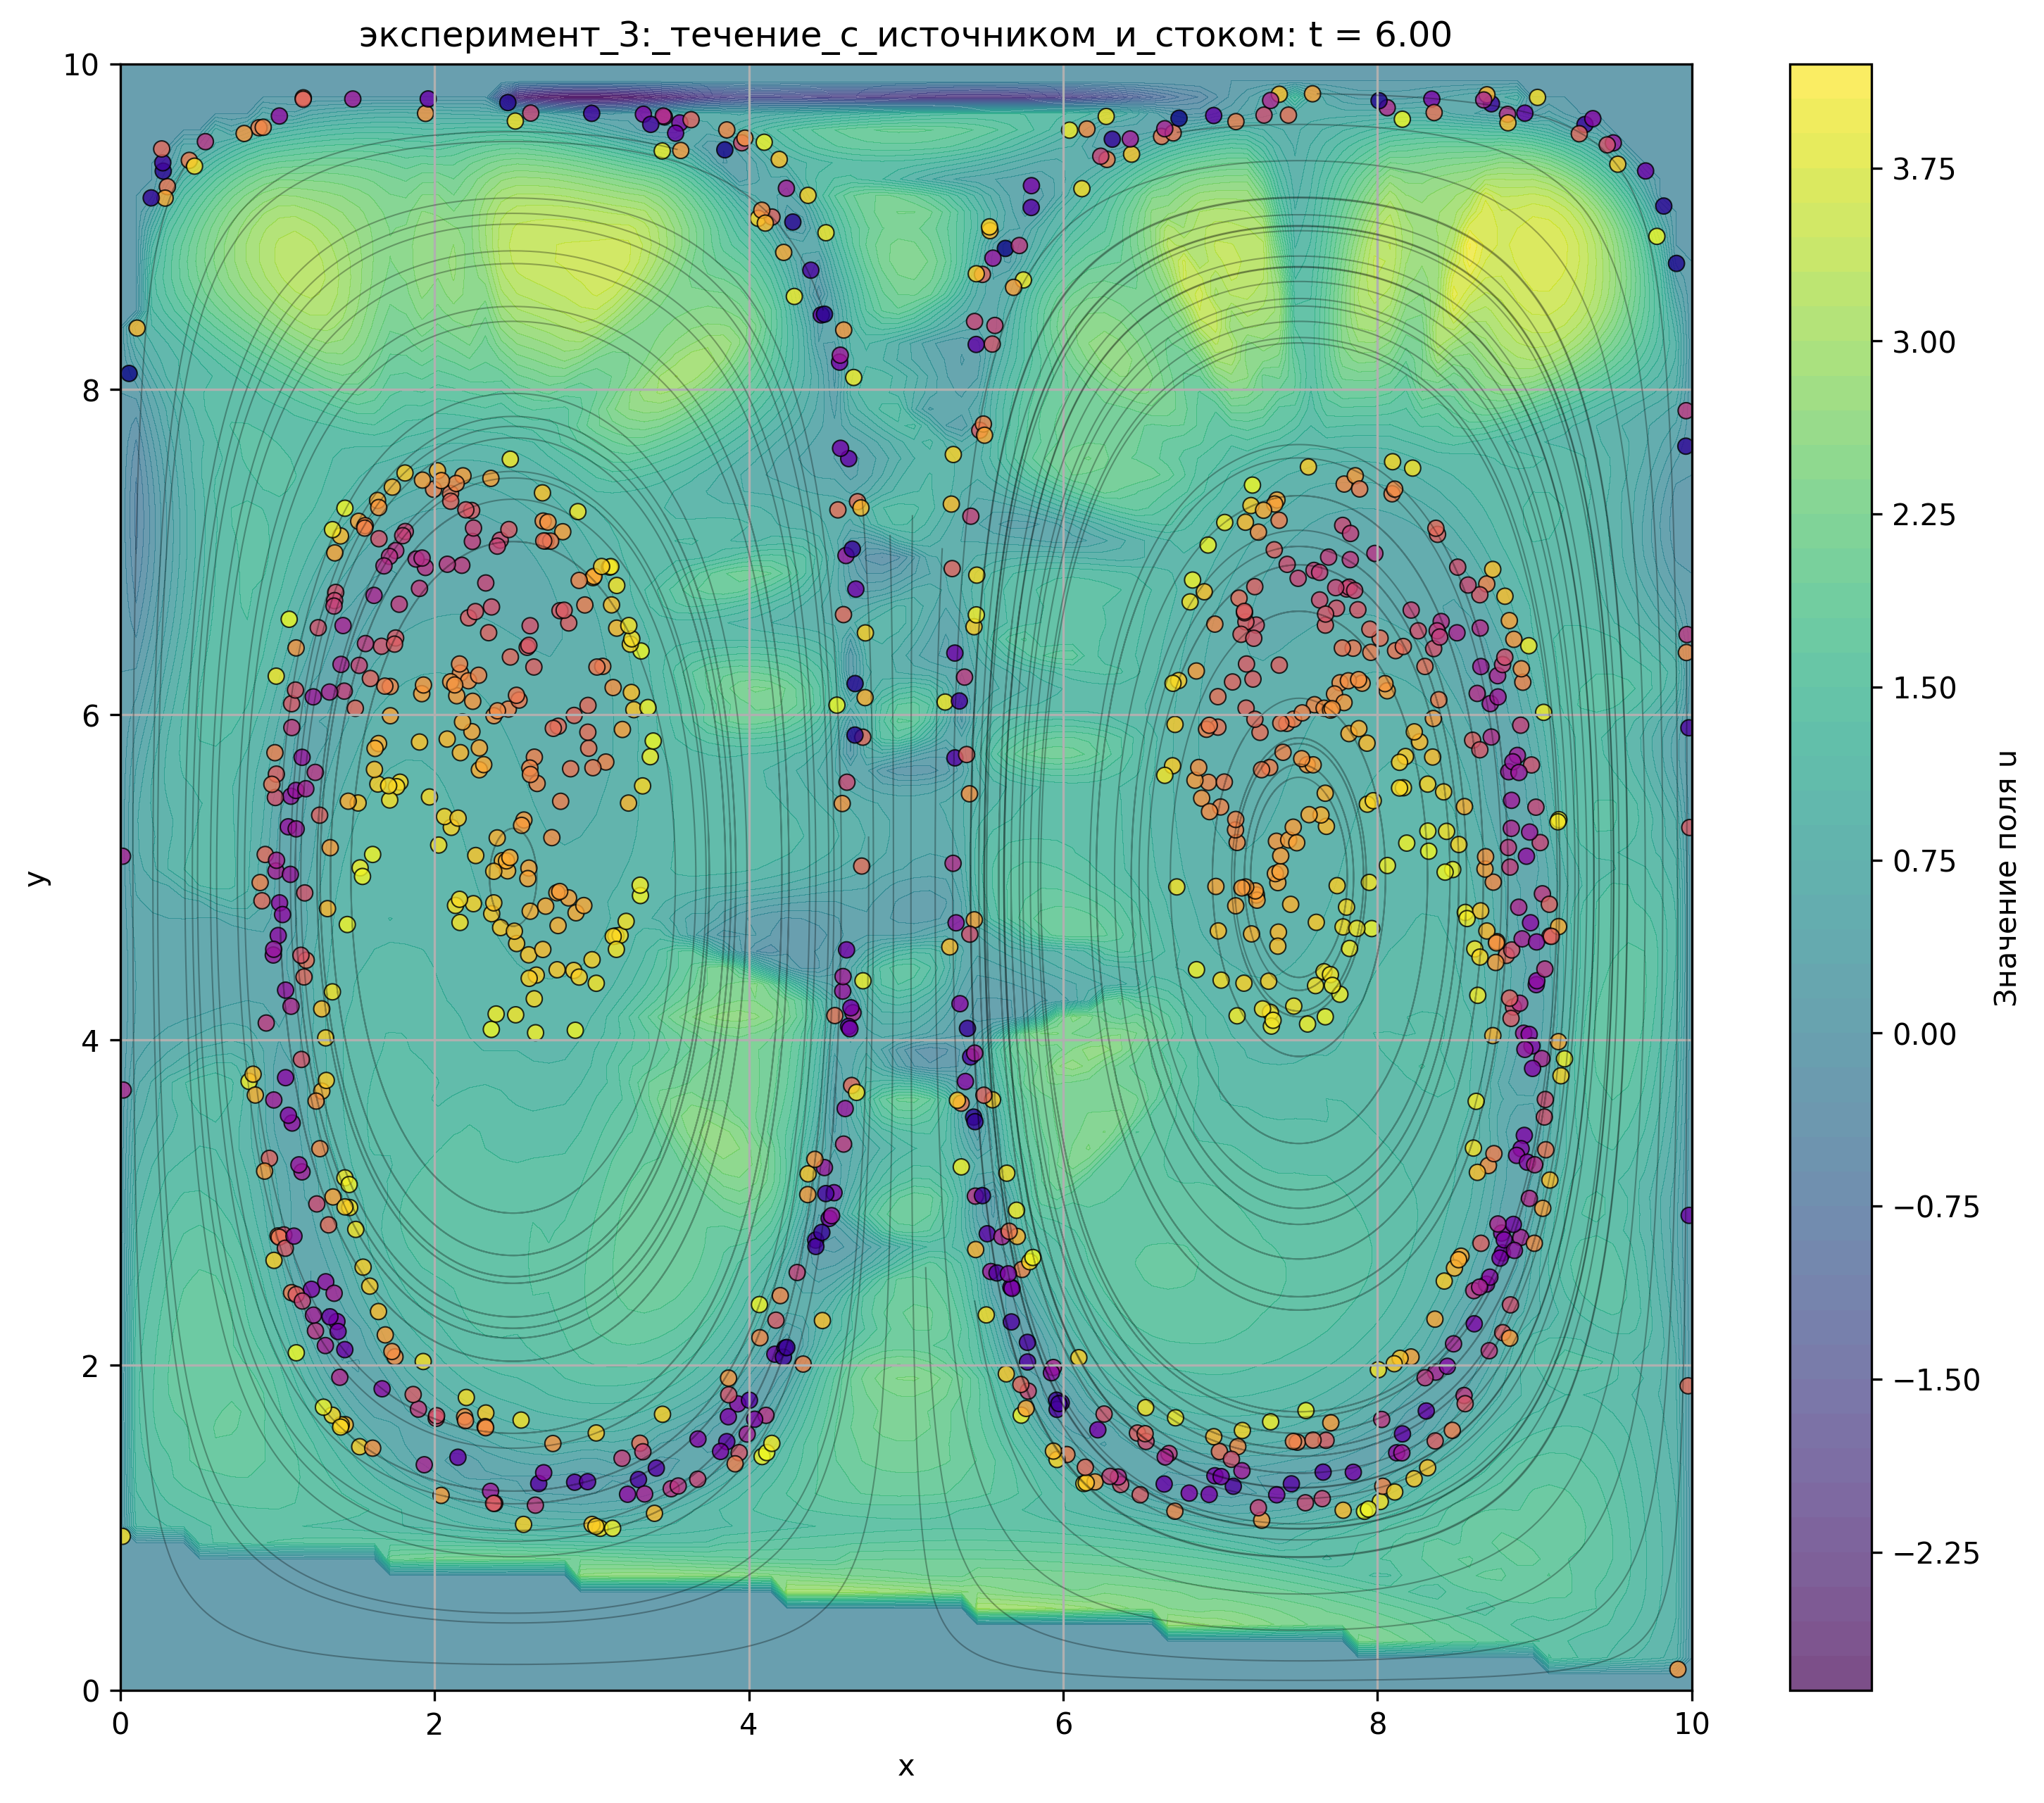
\includegraphics[width=0.6\textwidth]{imgs/lg/эксперимент_3:_течение_с_источником_и_стоком_t6.00.png}
	\caption{Скалярное поле в момент времени $t=6$ }
\end{figure}
\begin{figure}[h]
	\centering
	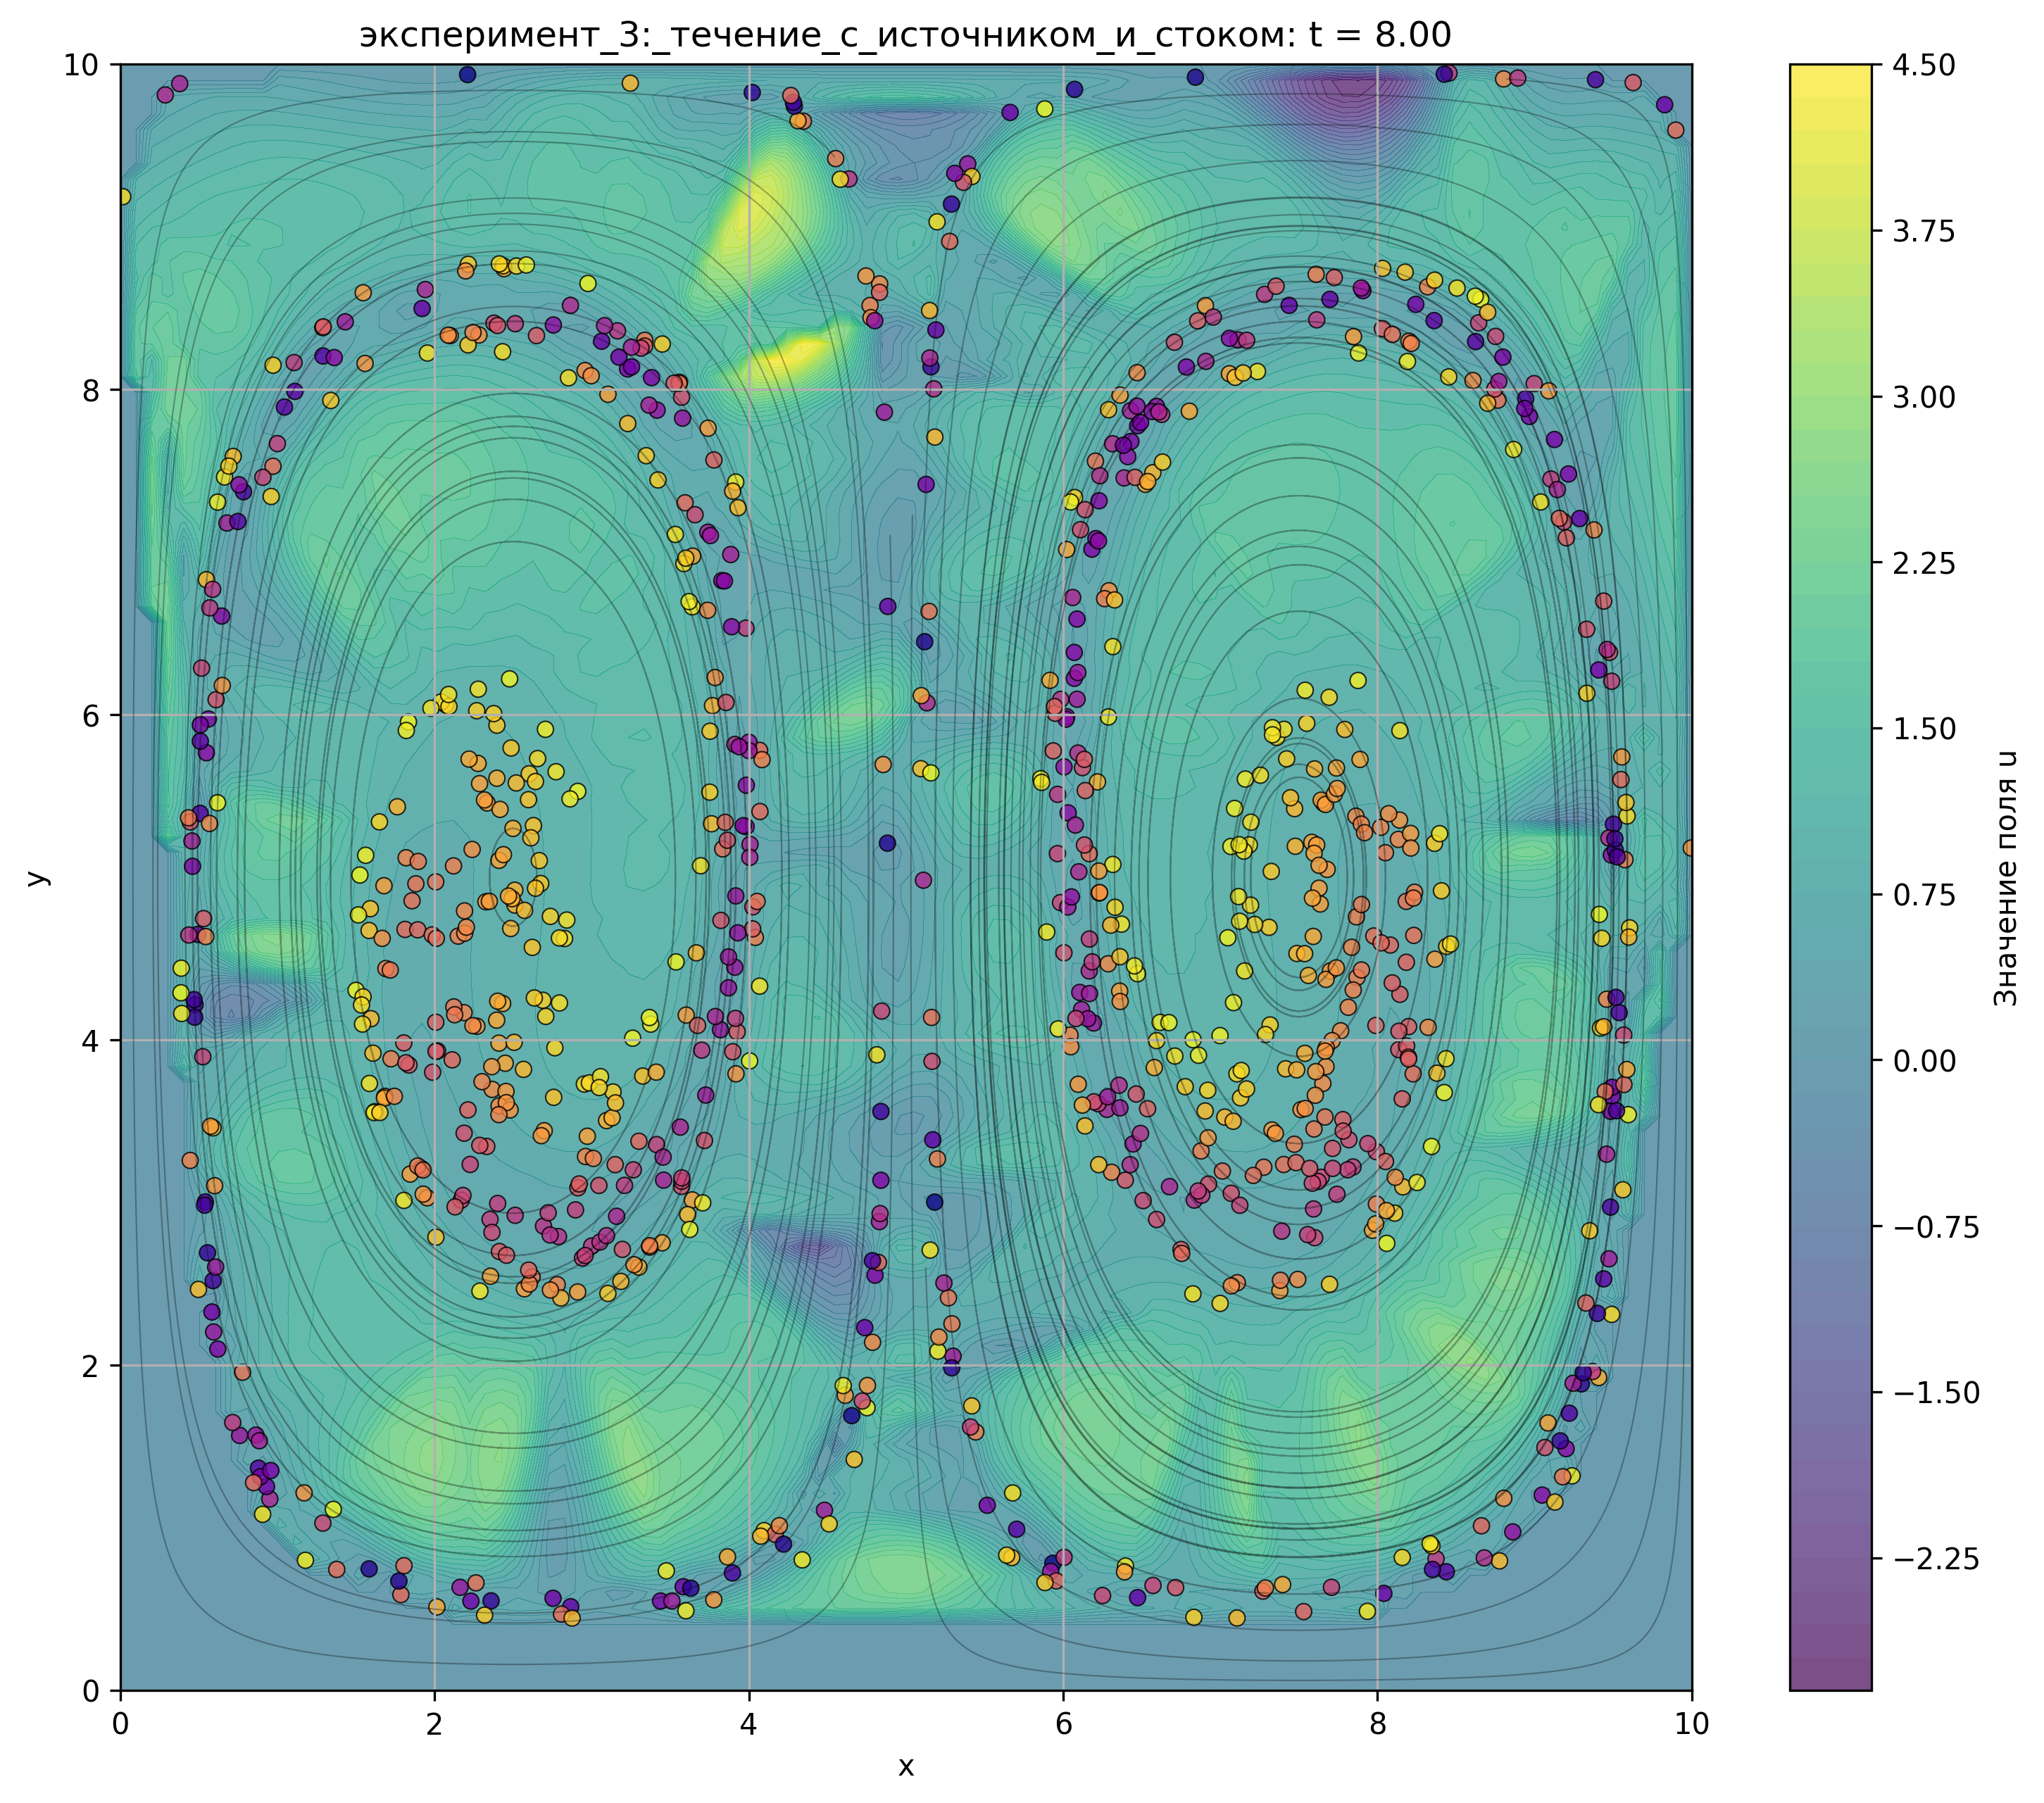
\includegraphics[width=0.6\textwidth]{imgs/lg/эксперимент_3:_течение_с_источником_и_стоком_t8.00.png}
	\caption{Скалярное поле в момент времени $t=8$}
\end{figure}